\documentclass[a4paper,12pt]{article}

\usepackage[utf8]{inputenc}
\usepackage[T1]{fontenc}
\usepackage[dutch]{babel}

\usepackage{graphicx}			%gif/jpeg/... images
\usepackage{subfigure}
\usepackage{a4wide}				%fullpage
%\usepackage{fancyhdr}
%\pagestyle{fancy}

%\usepackage{chappg}			%Number pages by chapter

%%%
\usepackage{float}
\floatstyle{boxed}
\newfloat{listing}{h}{lgr}
\floatname{listing}{Listing}
%%%

\begin{document}

\title{
	\textbf{Voorstel Layoutalgoritme} \\ 
	\large{Het Laatste Nieuws}}
	\author{\textbf{Cronos, XT-i}}

\maketitle
%\tableofcontents

	\section{Voorbeeld}
Onderstaande figuur toont \textit{een} mogelijke layout, vertrekkende van het XML bestand. De rekentijd is 6,22 seconden. Linksonder de tweede pagina staat een advertentie.
	
\begin{figure}[htp]
	\centering
	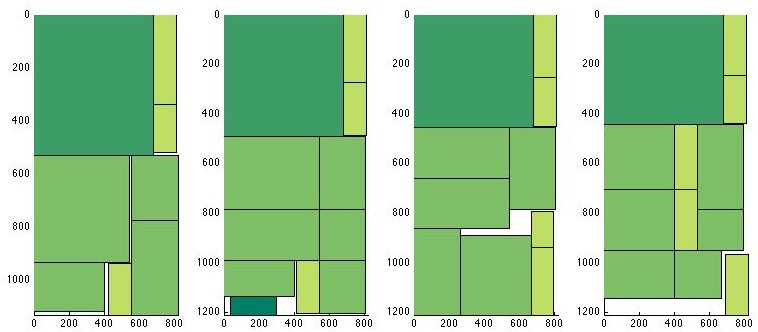
\includegraphics[width=\textwidth]{layout2}
	\caption{Een mogelijke layout}
	\label{fig:vb}
\end{figure}

	\section{Idee}
Artikels beginnen niet willekeurig op een pagina. Artikels beginnen in een hoek van de pagina of aan de hoek van een ander artikel. Dit zorgt voor een layout waar intrinsiek al weinig whitespace overblijft.

De huidige heuristiek zorgt voor een maximale inpassing. De artikels worden één voor één ingepast, waarbij in elke stap wordt geopteerd voor het artikel dat voor de \textit{beste} inpassing zorgt.

	\section{Algoritme}
De pagina is een rechthoek met een bepaalde breedte en hoogte. Artikels zijn rechthoeken met een bepaalde breedte en hoogte en hebben meerdere layouts.

Artikels worden aangehecht aan een \textit{ankerpunt}. Een artikel kan aan een ankerpunt worden aangehecht op 4 mogelijke manieren: rechtsonder, rechtsboven, linksonder, linksboven.

\begin{figure}[htp]
	\centering
	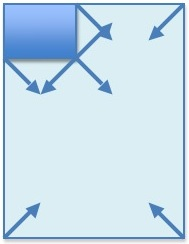
\includegraphics[width=3 cm]{ankerpunten}
	\caption{Een pagina met 1 artikel, de 6 ankerpunten met elk de mogelijke richtingen.}
	\label{fig:vb}
\end{figure}

Het algoritme is een soort Greedy Search\footnote{Best first}. Andere zoekalgoritmes zouden ook mogelijk zijn, bijvoorbeeld A*, mits een goede heuristiek gevonden kan worden. De stappen die worden doorlopen zijn:
\begin{enumerate}
	\item[] Start met lege paginas. Lege paginas hebben 4 ankerpunten: de 4 hoekpunten. Voeg eventuele advertenties toe per pagina. Advertenties hebben geen ankerpunten\footnote{Om te vermijden dat het eerste artikel niet linksboven tegen de rand, maar tegen de advertentie wordt geplaatst}.
	\item Zoek het artikel met de hoogste heuristische score (inpassingsgraad; zie sectie \ref{sec:heur}). \textit{In het geval van het eerste artikel op de pagina wordt het grootste artikel geplaatst omdat dit de grootste inpassing kan realiseren.}
	
	\begin{enumerate}
		\item Kies een (mogelijk) artikel.
		\item Kies een (mogelijke) pagina.
		\item Kies een (mogelijke) layout van het artikel die past op de pagina.
		\item Kies een (mogelijk) ankerpunt van de pagina.
		\item Kies een (mogelijke) richting van het ankerpunt waarbij de plaatsing van het artikel volledig op de pagina kan en waar geen overlappig gebeurt met andere artikels.
\newpage
		\item Contoleer of de huidige plaatsing overeenkomt met de business rules. Momenteel zijn geimplementeerd:
			\begin{itemize}
				\item Kopstukken beginnen enkel tegen de bovenste paginarand.
				\item Artikels met voorkeursplaatsing vooraan mogen niet op de achterste pagina geplaatst worden. Artikels met voorkeursplaatsing achteraan mogen niet op de voorste pagina geplaatst worden.
			\end{itemize}
		\item Bereken de score van deze plaatsing volgens de heuristiek.
		\item Overloop de volgende mogelijkheden: een ander(e) mogelijk(e) richting, ankerpunt, layout, pagina, artikel.
	\end{enumerate}
	
	\item Plaats het gevonden artikel (op de in stap 1 bepaalde pagina, layout, ankerpunt en richting). Genereer 4 nieuwe ankerpunten (de 4 hoekpunten van het artikel) en voeg deze toe aan de pagina.
	
	\item Ga naar stap 1.
\end{enumerate}
	\section{Heuristiek}
	\label{sec:heur}
Een mooie layout is weinig willekeurig en laat weinig witte ruimte over. Dit kan gekwanticifeerd worden met de inpassing: hoe goed past een bepaald artikel in een (onvolledige) layout.

De heuristiek meet de lengte van de zijden die tegen de paginarand of een ander artikel liggen. Figuur \ref{badlayoutbetter} toont een layout die beter is dan figuur \ref{badlayout}. In de rechterfiguur zijn de aaneengesloten zijden opmerkelijk groter.

Deze vaststelling is de basis voor de heuristiek.

\begin{figure}[htp]
  \begin{center}
    \subfigure[Een layout zonder inpassingsheuristiek]
    	{
			\label{badlayout}
			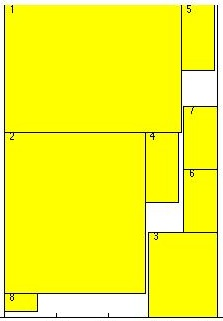
\includegraphics[scale=0.45]{badlayout}
		}
    \subfigure[Een layout met inpassingsheuristiek]
    	{
			\label{badlayoutbetter}
			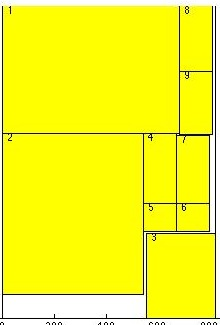
\includegraphics[scale=0.45]{badlayoutbetter}
		}
  \end{center}
  \caption{De zin van een inpassingsheuristiek}
  \label{fig:edge}
\end{figure}

Artikels die even hoog of breed zijn en naast elkaar liggen geeft ook een esthetische surplus. Als aan deze zijden een hogere heuristische score wordt toegekend, geeft het algoritme de rechterlayout.

\begin{figure}[htp]
	\centering
	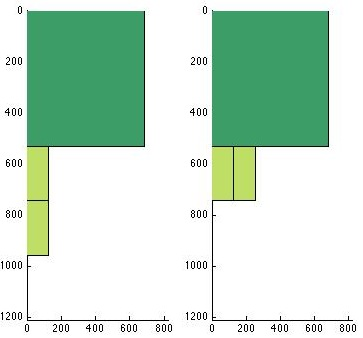
\includegraphics[width=8 cm]{gelijkezijden}
	\caption{Een mogelijke layout. Rechts wordt een hogere score toegekend voor even lange zijden.}
	\label{fig:vb}
\end{figure}
	
	\section{Relevante vragen}
Figuur \ref{tweeopties} toont twee opties. De bovenste figuur \ref{figa} toont een layout gegenereerd aan de hand van de heuristiek met de aanpassing ter bevoordeling van zijden die even groot zijn. Indirect worden grote artikels bevoordeeld door plaatstekort.

In het zoekproces zal een groot artikel op een deels lege pagina immers een grotere insluiting kunnen realiseren dan een klein artikel, en zal dus eerst geplaatst worden. Een klein artikel zal pas aan bod komen als de pagina eventueel al vol staat.

De onderste figuur \ref{figb} toont de eerste layout die aan alle voorwaarden voldoet. Er komt geen heuristiek aan te pas. De layout is eerder chaotisch en er is veel whitespace die opgelost zou kunnen worden door te schuiven met de artikels. Grote artikels hebben hier geen voordeel op de kleine artikels. Wel hebben artikels die eerder in het XML bestand staan, voordeel.

\begin{itemize}
	\item Hoe ziet een goede layout eruit? Veel gelijke zijden of juist niet?
	\item Moeten kleine artikels meer bevoordeeld worden?
	\item Welke artikels zijn belangrijk?
	\item ...
\end{itemize}

	
\begin{figure}[htp]
  \begin{center}
    \subfigure[Inpassingsheuristiek. Artikels met even grote zijde worden bevoordeeld. Indirect worden grote artikels bevoordeeld.]
    	{
			\label{figa}
			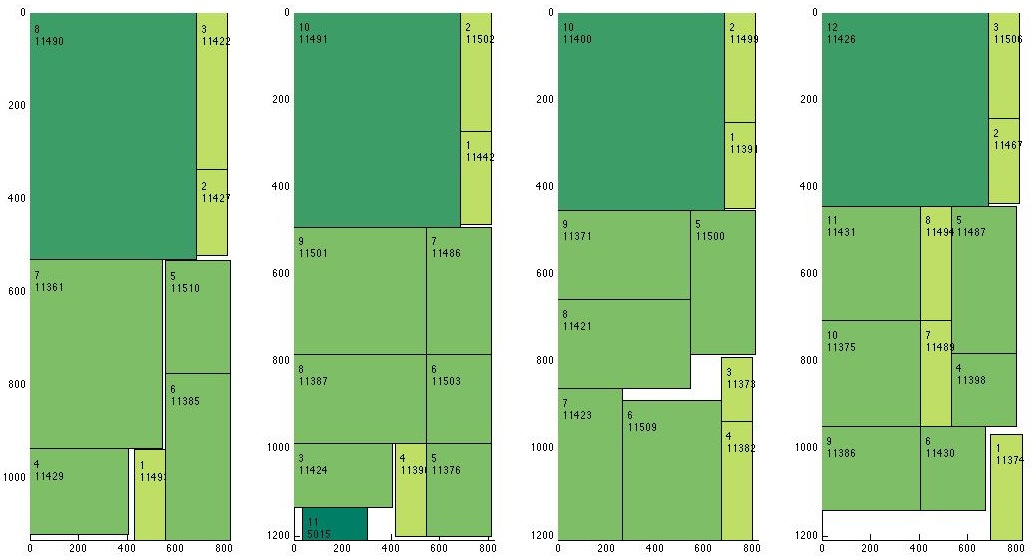
\includegraphics[width=\textwidth]{check}
		}
    \subfigure[Geen heuristiek (eerste mogelijke oplossing). Bemerk de hoeveelheid en de chaotische aard van de whitespace. Bemerk het aantal kleine artikels. Volgorde in XML is bepalend.]
    	{
			\label{figb}
			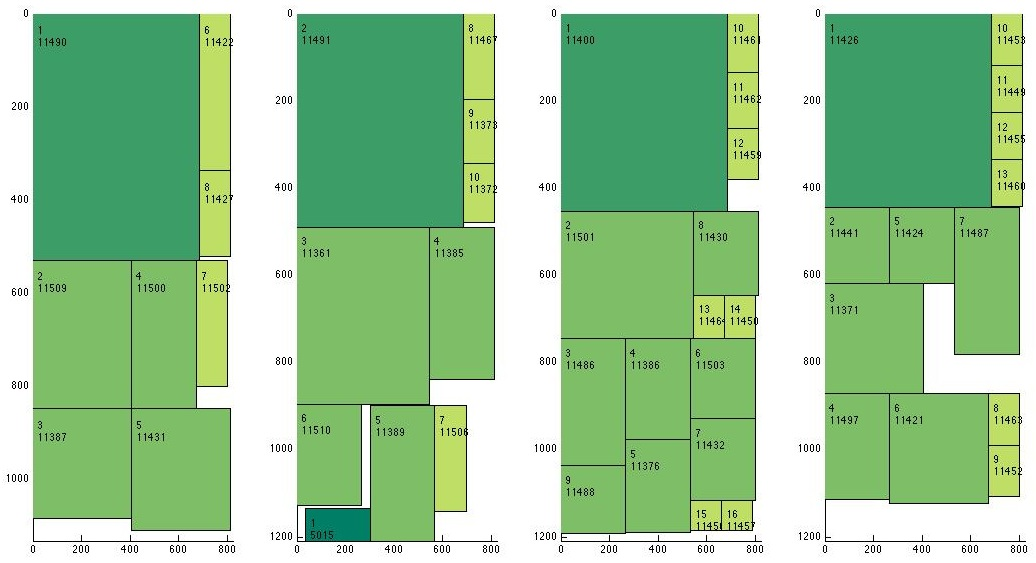
\includegraphics[width=\textwidth]{sol1}
		}
  \end{center}
  \caption{Twee opties}
  \label{tweeopties}
\end{figure}

%\chapter{Inleiding}
%	\section{Administratieve Gegevens}
%	
%\begin{table}[htbp]
%  \begin{tabular}{rl}
%    Naam Student: 	& Wouter Van Ranst \\
%	Studiejaar: &	$1^{e}$ Master Computerwetenschappen -- Artificiele Intelligentie \\	\\
%	Naam Bedrijf:	& Chronos NV, XT-i Extreme Implementations \\
%    Adres Bedrijf:	& Veldkant 35D, 2550 Kontich \\
%	\\
%	Naam Stagebegeleider:	& Günther Van Roey, Tim Goffings \\
%	Stageperiode:	& 1 augustus -- 22 augustus, 3 september -- 9 september 2008
%  \end{tabular}
%\end{table}
%	
%	\section{Beschrijving van het bedrijf}

%\chapter{Verslag}
%	\section{Probleemstelling}
%De Vlaamse krant Het Laatste Nieuws\footnote{http://www.hln.be/}, wil zich in de toekomst meer toespitsen op regionaal nieuws. De krant wil de huidige 5 edities (Antwerpen, Limburg, West-Vlaanderen, Oost-Vlaanderen en Vlaams-Brabant) nog verder opdelen.

%De belangrijkste problemen die hierbij overkomen moeten worden zijn ten eerste het opstellen van de layout (het plaatsen van de artikels op de pagina's) en ten tweede het snel kunnen drukken van deze verschillende edities.

%Het laatste probleem is opgelost met digitale drukpersen waarbij het manueel verwisselen van drukplaten niet meer nodig is. Het eerste probleem blijft echter.

%Momenteel gebeurt het layouten manueel en neemt per editie ongeveer 5 uur in beslag. Als de eerste krant om 05h00 bezorgd moet worden, het drukken 4 uur duurt en het layouten 5 uur, dan kan het laatste artikel ten laatste om 8 uur 'savonds binnenkomen om de krant van de volgende dag te halen. Dit is verre van ideaal.
%\\ 
%\\
%HLN heeft eigenhandig een layoutalgoritme gemaakt maar dit levert, na 2 uur rekenwerk, matige layouts op die nog manueel moeten aangepast worden.

%	\section{Voorstellen}
%		\subsection{Fysiek layoutprobleem}
%In het vak \textit{Fysieke Logistiek}\footnote{H01R9A, 3e Bachelor Bedrijfsbeheer, Pintelon L.}.
%plant oppervlaktes, geen rechthoeken?	
%		
%		\subsection{Lineair Programma}
%Te complex?
%	
%		\subsection{Prolog en varianten}
%In het vak \textit{Advanced Programming Languages for A.I.}\footnote{H02A8A, 1e Master AI, Janssens G.} komen enkele moderne constraint solvers aan bod, gebouwd bovenop Prolog.

%			\subsubsection{Prolog}
%De ingebouwde backtracking van Prolog maakt dit heel geschikt voor een layoutalgoritme. Verschillende layouts kunnen gegenereerd worden d.m.v. backtracking zonder een grote overheadkost.
%			
%			\subsubsection{CHR}
%Traag (cfr. Kuromasu/Sudoku)
%			
%			\subsubsection{ECLiPSe}
%pure prolog: indexen van matrix/array moeilijk > eclipse
%		
%		\subsection{Java}
%te veel overhead door objecten. geen native backtrack support.

%	\section{Invoer}
%De door de journalisten geschreven artikels worden door QuarkXPress gerenderd tot verschillende mogelijke vormen (verschillende hoogte/breedte, andere kop, ander lettertype, ...). Dit resulteert in een reeks `rechthoeken'. Samen met de grootte van elke pagina en eventuele ruimte voor advertenties wordt dit geexporteerd naar XML. Een ingekorte versie van een dergelijk XML bestand staat in listing \ref{listing:inXML} (pagina \pageref{listing:inXML}).

%			\subsubsection{Pagina's}
%De belangrijkste gegevens van de \verb|page| nodes, zijn \verb|usewidth| en \verb|useheight|. Dit zijn respectievelijk de bruikbare breedte en hoogte van de pagina. Merk op dat dit kan verschillen van pagina tot pagina. Verder is er ook het \verb|id| van de pagina, een uniek nummer per pagina.

%			\subsubsection{Artikels}
%De belangrijkste gegevens van de \verb|artikel| nodes, zijn \verb|type|, \verb|plaatsing|. De belangrijkste gegevens van de \verb|artlayout| subnodes, zijn \verb|width|, \verb|height|.

%\paragraph{Type} Er zijn 3 types. \verb|Kopstuk| betekent dat het artikel enkel geplaatst mag worden tegen de bovenkant. \verb|Normaal| betekent een normaal artikel en \verb|Kortje| betekent een klein artikel (merk op het verschil in width en height), typisch met maar 1 layoutmogelijkheid.

%\paragraph{Plaatsing} Er zijn 3 plaatsingsmogelijkheden. Een artikel met een plaatsing\verb|V| moet \textit{vooraan} in de regionale sectie geplaatst worden. Een artikel met plaatsing \verb|M| in het \textit{midden} en een artikel met plaatsing \verb|A| \textit{achteraan}.

%\paragraph{Artlayout} Een artikel heeft één of meerdere layouts. Elke layout heeft een uniek (over alle artikels) nummer \verb|id| dat de layout identificeert, een \verb|width| en een \verb|height|, dewelke de afmetingen van de rechthoek waarbinnen het artikel geplaatst zal worden, bepalen.

%	\section{Algoritmes}
%		\subsection{Versie 1}
%			\subsubsection{Algoritme}
%Elke pagina wordt gediscretiseerd in een paar rijen en kolommen. Voor elk artikel wordt berekend hoeveel rijen en kolommen het zal innemen. 
%\begin{enumerate}
%	\item Kies het te plaatsen artikel. Dit is hier eenvoudigweg in volgorde van het invoerbestand. 
%	\item Kies een layout van het artikel. Dit is hier eenvoudigweg in volgorde van het invoerbestand.
%	\item Zoek op de pagina een vrije ruimte waar het artikel met de layout (met bepaalde afmetingen) geplaatst kan worden, rekening houdend met plaatsingsregels\footnote{Bijvoorbeeld: Kopstukken mogen enkel op de eerste rij geplaatst worden. Dit is de enige geimplementeerde regel.}. Indien er geen ruimte is, ga naar het volgende artikel (stap 1).
%	\item Wijs de ruimte op de pagina toe aan het artikel. Ga naar het volgende artikel (stap 1).
%\end{enumerate}
%			
%			\subsubsection{Implementatie}
%\paragraph{Geheugenstructuur toegewezen artikels} De gediscretiseerde pagina (met aantal kolommen C en aantal rijen R) wordt in het geheugen bijgehouden als een CxR matrix. De elementen van de matrix zijn op dit ogenblik vrije variabelen. Bij de toewijzing van een artikel aan de pagina krijgen de elementen die binnen de rechthoek vallen de waarde van het artikel id. De representatie in het geheugen heeft dus een visuele betekenis. Als de matrix wordt uitgeprint is de layout zichtbaar. Een voorbeeld staat in listing \ref{listing:layouteersteopl}.

%\paragraph{Zoek vrije ruimte} Het zoeken naar een vrije ruimte op de pagina gebeurt als volgt. Kies een startcoordinaat (hier (1,1) van de discrete pagina). Bereken de afmetingen van de rechthoek. Controleer of er overlap is met een ander, vroeger geplaatst artikel. Indien er geen overlap is mag het artikel hier geplaatst worden. Indien er wel overlap is, probeer dan de volgende coordinaat. De matrix wordt doorlopen van links naar rechts, en van boven naar onder.
%			
%			\subsubsection{Uitvoering}
%Met een grid van 10x15 wordt na 0,01s\footnote{Apple MacBook, Intel Core 2 Duo 2,16 GHz, 3 GB RAM, OS X Leopard 10.5.4, ECLiPSe 5.10} de eerste oplossing uitgeprint. De stappen dat het algoritme uitprint zijn weergegeven in listing \ref{listing:opeenvolgendegeplaatsteartikels} (pagina \pageref{listing:opeenvolgendegeplaatsteartikels}). De gegenereerde layout is weergegeven in listing \ref{listing:layouteersteopl}. De volgende oplossing, berekend na 0,05s meer, verschuift het laatst geplaatste artikel (met id 30902) één eenheid naar rechts. De gegenereerde layout is weergegeven in listing \ref{listing:volgendeopl}.
%\\
%\\
%Onderstaande tabel toont voor verschillende dimensies de tijd tot het berekenen van respectievelijk de eerste, tweede en zestigste oplossing.
%      
%\begin{table}[h]
%  \centering
%  \begin{tabular}{c|ccc}
%	Dimensie (BxH) & 1e Opl. & 2e Opl. & 60e Opl. \\
%	\hline
%    10x15 & 0,01s & 0,06s & 0,75s \\ 
%    20x30 & 0,03s & 0,06s & 1,63s \\ 
%    80x120 & 0,22s & 0,42s & 11,48s \\ 
%  \end{tabular}
%  \caption{Uitvoeringstijden voor verschillende dimensies}
%  \label{tab:exectimesalg1}
%\end{table}
%				
%			\subsubsection{Conclusie}
%Dit algoritme genereert voor de gegeven artikels elke mogelijke layout, ongeacht of deze esthetisch aanvaardbaar is of niet. Een goede layout zal naar alle waarschijnlijkheid pas laat in het zoekproces tevoorschijn komen. Om een goede bladvulling te bekomen moet ook het discretisatiegrid groot genoeg gedimensioneerd worden (de afmetingen van artikels worden naar boven afgerond en zal er bij een klein grid dus veel \textit{verloren} ruimte zijn). Er moeten dus veel layouts op een groot grid berekend worden. Zoals de laatste rij van tabel \ref{tab:exectimesalg1} laat zien kan dit onaanvaardbaar lang duren. 

%In het voorbeeld van listing \ref{listing:opeenvolgendegeplaatsteartikels} worden 5 artikels geplaatst op een 10x15 grid. De orde van het aantal plaatsingsmogelijkheden\footnote{Aantal plaatsingsmogelijkheden per artikel: $(GridWidth-ArtWidth+1) \cdot (GridHeight-ArtHeight+1)+1$, Toegepast op voorbeeld: $29 \cdot 53 \cdot 92 \cdot 118 \cdot 118 = 2\cdot10^{9}$} is $10^{9}$. Gezien de tijd om 60 mogelijkheden te berekenen, zal het berekenen van deze mogelijkheden orde 100 dagen duren.

%De oorzaak hiervoor is de geheugenstructuur voor toegewezen artikels, en het zoeken naar vrije ruimte om een artikel te plaatsen, dewelke op inefficiente wijze gebeuren.

%		\subsection{Versie 2}
%Het voorgaande algoritme kan op verscheidene punten verbeterd worden.
%\begin{itemize}
%	\item Keuze van te plaatsen artikel
%	\item \textit{Verloren} ruimte door (te) klein grid
%	\item Zoeken naar vrije ruimte, keuze van beginpunt
%	\item Geheugenstructuur geplaatste artikels
%	\item Intelligent zoeken naar een esthetische layout
%\end{itemize}

%keuze van beginpunt: artikels beginnen niet random, maar op ankerpunt

%Zoeken naar vrije ruimte, keuze van beginpunt: zoekruimte verkleint drastisch
%		
%	\section{Embedding}

%\chapter{Relatie tussen stage en opleiding}
%(minstens 1 pag, max 3)

%\chapter{Conclusie}

%\appendix

%\chapter{Invoer}
%	\section{XML}

%\begin{listing}
%	\begin{verbatim}
%	<all>
%	  <pages>
%	    <page id="5001" isleft="0" artikelslinks="false" margex="35.4325" 
%	          margey="150.630644" usewidth="822.034" useheight="1132.025856"></page>
%	    [...]
%	    <page id="4995" isleft="1" artikelslinks="true" margex="35.4325" 
%	          margey="73.8328262" usewidth="822.034" useheight="1208.8236738">
%	      <ad id="5015" x="35.433" y="1208.957" width="266.452"  height="73.7"/>
%	    </page>
%	  </pages>
%	  <artikels>
%	    <artikel id="11490" type="Kopstuk" plaatsing="V">
%	      <artlayout id="31075" width="683.139" height="529.0"/>
%	      <artlayout id="31074" width="683.139" height="529.0"/>
%	      [...]
%	      <artlayout id="31073" width="544.243" height="625.0"/>
%	    </artikel>
%	    [...]
%	    <artikel id="11509" type="Normaal" plaatsing="M">
%	      <artlayout id="31057" width="405.348" height="319.0"/>
%	      [...]
%	      <artlayout id="31053" width="266.452" height="436.0"/>
%	    </artikel>
%	    [...]
%	    <artikel id="11390" type="Kortje" plaatsing="A">
%	      <artlayout id="30899" width="127.557" height="214.0"/>
%	    </artikel>
%	  </artikels>
%	</all>
%	\end{verbatim}
%  \caption{Invoer XML bestand}
%  \label{listing:inXML}
%\end{listing}

%\chapter{Uitvoer}

%	\section{Algoritme 1}

%\begin{listing}
%	\begin{verbatim}
%		Page Size (WxH): [10, 15]
%		Placing: artikel(id(11490), type(kopstuk), plaatsing(m), 
%		   [layout(id(31073), width(7), height(9))])
%		Placed: 31073 [1, 7, 1, 9]  % ([StartX, StartY, EndX, EndY])
%		Placing: artikel(id(11387), type(normaal), plaatsing(v), 
%		   [layout(id(31042), width(7), height(3))])
%		Placed: 31042 [1, 7, 10, 12]
%		Placing: artikel(id(11488), type(normaal), plaatsing(m), 
%		   [layout(id(30945), width(4), height(3))])
%		Placed: 30945 [1, 4, 13, 15]
%		Placing: artikel(id(11391), type(kortje), plaatsing(a), 
%		   [layout(id(31052), width(2), height(3))])
%		Placed: 31052 [8, 9, 1, 3]
%		Placing: artikel(id(11384), type(kortje), plaatsing(a), 
%		   [layout(id(30902), width(2), height(3))])
%		Placed: 30902 [8, 9, 4, 6]
%	\end{verbatim}
%  \caption{Opeenvolgende geplaatste artikels}
%  \label{listing:opeenvolgendegeplaatsteartikels}
%\end{listing}

%\begin{listing}
%	\begin{verbatim}
%		 31073 31073 31073 31073 31073 31073 31073 31052 31052 .....
%		 31073 31073 31073 31073 31073 31073 31073 31052 31052 .....
%		 31073 31073 31073 31073 31073 31073 31073 31052 31052 .....
%		 31073 31073 31073 31073 31073 31073 31073 30902 30902 .....
%		 31073 31073 31073 31073 31073 31073 31073 30902 30902 .....
%		 31073 31073 31073 31073 31073 31073 31073 30902 30902 .....
%		 31073 31073 31073 31073 31073 31073 31073 ..... ..... .....
%		 31073 31073 31073 31073 31073 31073 31073 ..... ..... .....
%		 31073 31073 31073 31073 31073 31073 31073 ..... ..... .....
%		 31042 31042 31042 31042 31042 31042 31042 ..... ..... .....
%		 31042 31042 31042 31042 31042 31042 31042 ..... ..... .....
%		 31042 31042 31042 31042 31042 31042 31042 ..... ..... .....
%		 30945 30945 30945 30945 ..... ..... ..... ..... ..... .....
%		 30945 30945 30945 30945 ..... ..... ..... ..... ..... .....
%		 30945 30945 30945 30945 ..... ..... ..... ..... ..... .....
%	\end{verbatim}
%  \caption{Layout van de eerste oplossing}
%  \label{listing:layouteersteopl}
%\end{listing}

%\begin{listing}
%	\begin{verbatim}
%		Placed: 30902 [9, 10, 4, 6]

%		 31073 31073 31073 31073 31073 31073 31073 31052 31052 .....
%		 31073 31073 31073 31073 31073 31073 31073 31052 31052 .....
%		 31073 31073 31073 31073 31073 31073 31073 31052 31052 .....
%		 31073 31073 31073 31073 31073 31073 31073 ..... 30902 30902
%		 31073 31073 31073 31073 31073 31073 31073 ..... 30902 30902
%		 31073 31073 31073 31073 31073 31073 31073 ..... 30902 30902
%		 31073 31073 31073 31073 31073 31073 31073 ..... ..... .....
%		 31073 31073 31073 31073 31073 31073 31073 ..... ..... .....
%		 31073 31073 31073 31073 31073 31073 31073 ..... ..... .....
%		 31042 31042 31042 31042 31042 31042 31042 ..... ..... .....
%		 31042 31042 31042 31042 31042 31042 31042 ..... ..... .....
%		 31042 31042 31042 31042 31042 31042 31042 ..... ..... .....
%		 30945 30945 30945 30945 ..... ..... ..... ..... ..... .....
%		 30945 30945 30945 30945 ..... ..... ..... ..... ..... .....
%		 30945 30945 30945 30945 ..... ..... ..... ..... ..... .....
%	\end{verbatim}
%  \caption{Layout van de volgende oplossing (bemerk verplaatst artikel 30902)}
%  \label{listing:volgendeopl}
%\end{listing}

\end{document}